\lab{Data Visualization}{Data Visualization}
\label{lab:DataVis}
\objective{Correctly presenting and interpreting data with visualizations is both a science and an art.
% Indeed, effectively communicating complex relationships through data visualization is crucial to gaining the understanding needed to make important and difficult decisions.
In this lab we discuss and demonstrate the principles of good data visualization, including the key characteristics of good graphs, common mistakes, and how to avoid unethical visualizations.
\\ \indent We strongly recommend completing this lab as a Jupyter Notebook.}

\section*{The Importance of Visualizations} % =================================

Visualizations of data often reveal insights that may not immediately obvious from simple statistics.
The following data set, known as \emph{Anscombe's quartet}, is a famous example of the importance of graphing data.

\begin{table}[H]
\small{
\begin{tabular}{rr|rr|rr|rr}
    \multicolumn{2}{c|}{I}    & \multicolumn{2}{|c|}{II} &
    \multicolumn{2}{|c|}{III} & \multicolumn{2}{|c}{IV} \\
    \multicolumn{1}{c}{$x$}   & \multicolumn{1}{c|}{$y$} &
    \multicolumn{1}{|c}{$x$}  & \multicolumn{1}{c|}{$y$} &
    \multicolumn{1}{|c}{$x$}  & \multicolumn{1}{c|}{$y$} &
    \multicolumn{1}{|c}{$x$}  & \multicolumn{1}{c}{$y$} \\
    \hline
    10.0 & 8.04  & 10.0 & 9.14 & 10.0 & 7.46  & 8.0  & 6.58  \\
    8.0  & 6.95  & 8.0  & 8.14 & 8.0  & 6.77  & 8.0  & 5.76  \\
    13.0 & 7.58  & 13.0 & 8.74 & 13.0 & 12.74 & 8.0  & 7.71  \\
    9.0  & 8.81  & 9.0  & 8.77 & 9.0  & 7.11  & 8.0  & 8.84  \\
    11.0 & 8.33  & 11.0 & 9.26 & 11.0 & 7.81  & 8.0  & 8.47  \\
    14.0 & 9.96  & 14.0 & 8.10 & 14.0 & 8.84  & 8.0  & 7.04  \\
    6.0  & 7.24  & 6.0  & 6.13 & 6.0  & 6.08  & 8.0  & 5.25  \\
    4.0  & 4.26  & 4.0  & 3.10 & 4.0  & 5.39  & 19.0 & 12.50 \\
    12.0 & 10.84 & 12.0 & 9.13 & 12.0 & 8.15  & 8.0  & 5.56  \\
    7.0  & 4.82  & 7.0  & 7.26 & 7.0  & 6.42  & 8.0  & 7.91  \\
    5.0  & 5.68  & 5.0  & 4.74 & 5.0  & 5.73  & 8.0  & 6.89  \\
\end{tabular}}
\end{table}

Each section of Anscombe's quartet shares the following statistical properties:
\begin{itemize}
\setlength\itemsep{0em}
    \item The means are $9$ for $x$ and $7.5$ for $y$.
    \item The sample variances are $11$ for $x$ and $3.75$ for $y$.
    \item The correlation between $x$ and $y$ is $.816$.
    \item The linear least squares regression line is $y=\frac{1}{2}x+3$.
\end{itemize}

Despite these similarities, each section is quite different from the others.

\begin{problem} % Describe Anscombe's quartet.
The file \texttt{anscombe.npy} contains Anscombe's quartet in the same format as displayed above.
Plot each section of the quartet separately as a scatter plot.
Also plot the regression line $y = \frac{1}{2}x + 3$ on the domain $x\in[0,20]$ over each scatter plot.

Write a few sentences describing what makes each section unique.
\label{prob:anscombes-quartet}
\end{problem}

\section*{Principles of Good Data Visualization} % ============================

Effectively visualizing data involves technical expertise combined with design knowledge.
No visualization is perfect, but every good visualization must contain the following essential elements.

\begin{enumerate}
    \item \textbf{Clarity}.
    Visualizations should be self-explanatory.
    Always use specific titles and axis labels, and include units of measure.
    Use a legend or annotations where appropriate.

    \item \textbf{Simplicity}.
    A good visualization communicates everything that it needs to, but nothing more.
    Remove unnecessary or distracting elements of a graph, including 3-D effects or overly flashy colors.

    \item \textbf{Integrity}.
    Tell the truth, the whole truth, and nothing but the truth.
    It is almost always very easy to manipulate a visualization so that it supports a desired interpretation.
    Resist the temptation to morph a visualization into something that misrepresents the true nature of the data, even though that misrepresentation might support your hypotheses about the data.

    Every visualization should be presented together with information on who created it, where the data was obtained, how it was collected, whether it was cleaned or transformed, and whether there are conflicts of interest or possible biases present.
    Cite your sources.
\end{enumerate}

This list could be expanded, but virtually every good data visualization principle fits into these three categories in one way or another.

\section*{Improving Specific Types of Visualizations} % =======================

Data can be visualized in many forms and styles.
However, Most data sets are more naturally described with one type of visualization than another.
In the following sections, we explore how the plots we commonly use can be improved and refined.

\subsection*{Line Plots} % ----------------------------------------------------

A line plot connects ordered $(x,y)$ points with straight lines, and is therefore best for visualizing one or two ordered arrays, such as functional outputs over an ordered domain or a sequence of values over time.

\newpage

When creating a line plot, consider the following details.
%
\begin{itemize}
    \item What do the axes represent? How should they be labeled?
    \item Would a linear scale or a logarithmic scale most clearly reveal patterns?
    \item What should the window limits be?
    \item Is the line an appropriate thickness and color?
    \item Should each point be distinctly marked, or is a smooth line preferable?
    \item Should multiple lines be in the same plot, or in separate subplots?
\end{itemize}

The \emph{Chebyshev polynomials} are a family of orthogonal polynomials that are recursively defined as follows.
\[T_0(x) = 1 \qquad T_1(x) = x \qquad\qquad T_{n+1} = 2xT_n(x) - T_{n-1}(x)\]
NumPy's \li{polynomial} module has a convenient tool for constructing these and other important polynomials.%
\footnote{\li{numpy.polynomial} also has tools for computing other important polynomial families, including the Legendre, Hermite, and Laguerre polynomials.}
However, plotting several the polynomials on top of each other, especially with a legend, results in a very cluttered visual.

\begin{lstlisting}
>>> import numpy as np
>>> from matplotlib import pyplot as plt
>>> % matplotlib inline                     # Display notebook plots inline.

# Plot the first 9 Chebyshev polynomials in the same plot.
>>> T = np.polynomial.Chebyshev.basis
>>> x = np.linspace(-1, 1, 200)
>>> for n in range(9):
...     plt.plot(x, T(n)(x), label="n = "+str(n))
...
>>> plt.axis([-1.1, 1.1, -1.1, 1.1])        # Set the window limits.
>>> plt.legend()
\end{lstlisting}

\begin{figure}[H] % Chebyshev polynomials (bad example).
    \centering
    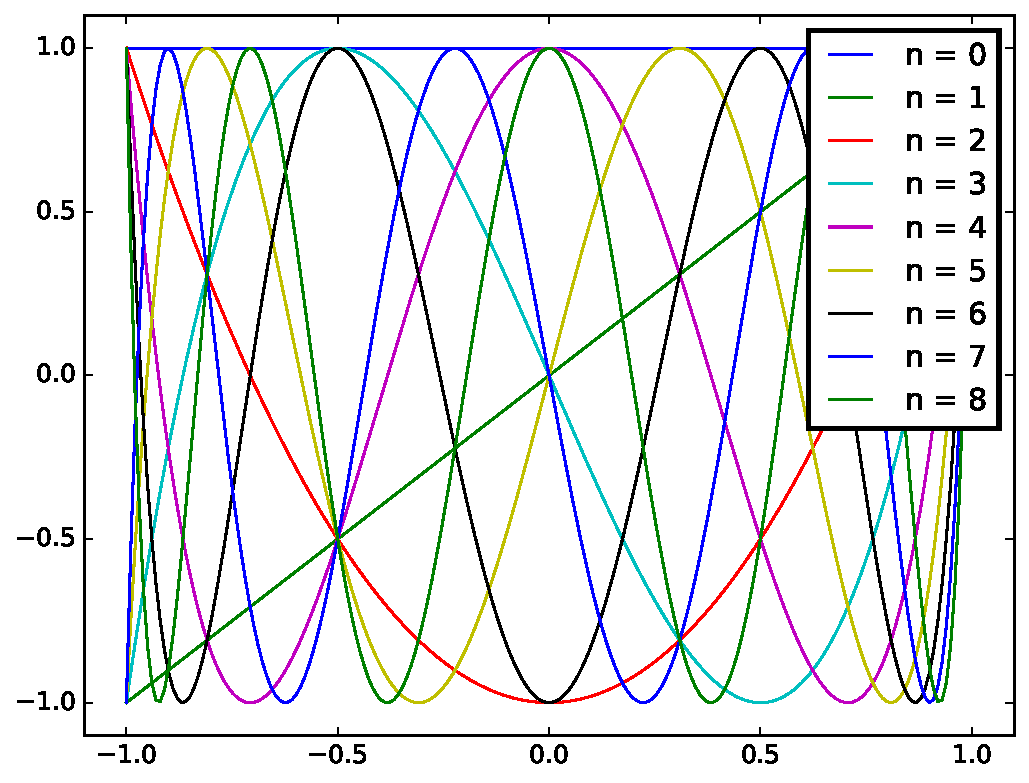
\includegraphics[width=.7\linewidth]{figures/chebyshev_bad.pdf}
\end{figure}

This line plot can be improved in several easy ways.
%
\begin{enumerate}
    \item
    Use subplots to split the visualization into smaller, comparable pieces.
    Instead of using a legend, give each subplot a title.
    This method, called \emph{small multiples}, was made famous by Edward Tufte.
    \item Increase the line thicknesses to 2 or 3 (the default is 1).
    \item Remove extra tick marks and axis labels.
\end{enumerate}

Matplotlib's \li{plt.tick_params()}, summarized below, controls which tick marks and labels are displayed.
%
\begin{table}[H]
\begin{tabular}{r|c|l}
    Argument & Options & Description
    \\ \hline
    \li{axis} & \li{'x'}, \li{'y'}, \li{"both"} & Axis on which to operate. \\
    \li{which} & \li{"major"}, \li{"minor"}, \li{"both"} & Operate on major or minor ticks.\\
    \li{color} & Any Matplotlib color & Tick color. \\
    \li{labelcolor} & Any Matplotlib color & Tick label color. \\
    \li{bottom}, \li{top}, \li{left}, \li{right} & \li{"on"}, \li{"off"} & Turn ticks on or off. \\
    \li{labelbottom}, \li{labeltop}, & \li{"on"}, \li{"off"} & Turn tick labels on or off. \\
    \li{labelleft}, \li{labelright} & &
\end{tabular}
\end{table}

\begin{lstlisting}
>>> for n in range(9):
...     plt.subplot(3, 3, n+1)
...     plt.plot(x, T(n)(x), lw=2)
...     plt.axis([-1.1, 1.1, -1.1, 1.1])
...
...     # Turn off extra tick marks and axis labels.
...     plt.tick_params(which="both", top="off", right="off")
...     if n < 6:                   # Remove x-axis label on upper plots.
...         plt.tick_params(labelbottom="off")
...     if n % 3:                   # Remove y-axis label on right plots.
...         plt.tick_params(labelleft="off")
...     plt.title("n = "+str(n))
\end{lstlisting}

\begin{figure}[H] % Chebyshev polynomials (bad example).
    \centering
    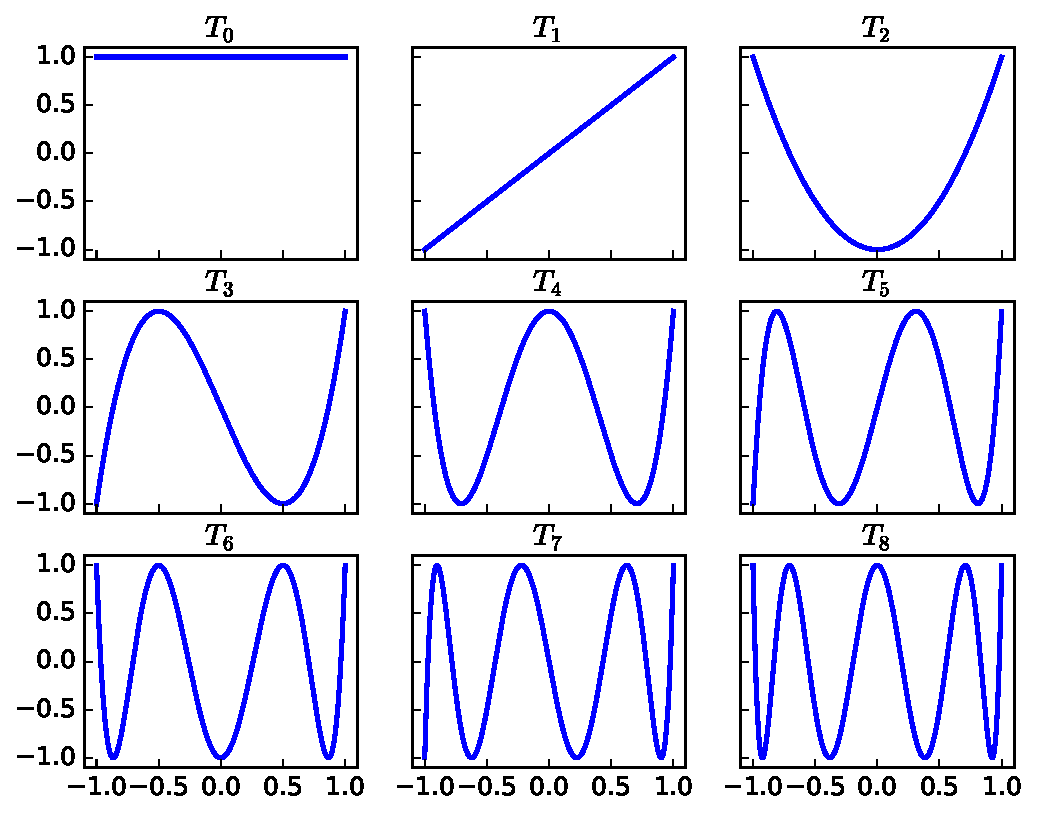
\includegraphics[width=.7\linewidth]{figures/chebyshev_good.pdf}
\end{figure}

\begin{info} % LaTex with Matplotlib text.
Matplotlib titles and annotations can be formatted with \LaTeX, a system designed for creating technical and scientific documents%
\footnote{See \url{http://www.latex-project.org/} for more information.}
(this lab manual, for example, is written in \LaTeX).
To do so, use an `r' before the string quotation mark) and surround the text with dollar signs.

For example, try replacing the final line of code in the previous example with the following line.

\begin{lstlisting}
...     plt.title(r"$T_{}(x)$".<<format>>(n))
\end{lstlisting}

The string's \li{<<format>>()} method inserts the input $n$ at the curly braces.
The title of the sixth subplot, instead of being ``n = 5,'' will then be ``$T_5(x)$.''
\end{info}

% TODO: Make sure the Bernstein polynomial notation is consistent with the book (it is consistent with Wikipedia currently)

\begin{problem} % Plot the Bernstein polynomials.
The $n+1$ Bernstein basis polynomials of degree $n$ are defined as follows.
\[b_{v,n} = {{n} \choose {v}} x^v (1-x)^{n-v},\qquad v = 0,\ 1,\ \ldots,\ n\]

Plot at least the first $10$ Bernstein basis polynomials ($n = 0,\ 1,\ 2,\ 3$) as small multiples on the domain $[0,1] \times [0,1]$.
Label the subplots for clarity, adjust tick marks and labels for simplicity, and set the window limits of each plot to be the same.
Consider arranging the subplots so that the rows correspond with $n$ and the columns with $v$.
\\(Hint: The constant ${{n} \choose {v}} = \frac{n!}{v!(n-v)!}$ is called the \emph{binomial coefficient} and can be efficiently computed with \li{scipy.special.binom()} or \li{scipy.misc.comb()}.)
\end{problem}

\subsection*{Scatter Plots} % -------------------------------------------------

A scatter plot draws $(x,y)$ points without connecting them.
Connecting the points would imply an order or relation between the points, so scatter plots are best for displaying data sets without a natural order, or where each point is a distinct, individual instance.

Consider the following questions when making a scatter plot.
Note that some of them are the same questions that should be asked when creating a line plot.
%
\begin{itemize}
    \item What do the axes represent? How should they be labeled?
    \item Would a linear scale or a logarithmic scale most clearly reveal patterns?
    \item What should the window limits be?
    \item Which marker is best? Are the markers an appropriate size and color?
\end{itemize}

A scatter plot can be drawn with either \li{plt.plot()} (specify a point marker such as \li{'.'}, \li{','}, \li{'o'}, or \li{'+'}) or \li{plt.scatter()}.
While \li{plt.plot()} is the more flexible function in general, \li{plt.scatter()} provides a few extra tools.
Most useful are the keywords \li{s} and \li{c}, which correspond to marker size and marker color, respectively.
Each keyword can either be a single entry or an array.
Using an array specifies the sizes or colors of each individual marker, allowing a scatter plot to have up to four dimensions of information.

\begin{comment}
% Window size, also should go later.
Figure \ref{fig:scatter_correlation} displays two scatter plots.
The first appears to have a weak correlation and the second appears to have a strong correlation.
However, the same data is being plotted and the only difference is the scale and window size.
Manipulating these can change your interpretation and should be done with careful consideration.
\end{comment}

Consider a collection of rectangular boxes where the lengths, widths, and heights are given.
A scatter plot of length against width mostly describes the sizes of the boxes; tying the third dimension (height) to the color of the points can provide the additional information.
Setting the marker size as the volume of the boxes also adds some depth to the visualization, though modifying both the color and the size might be considered overkill.

Since adjusting the marker size may lead to overlapping points, we specify the \emph{alpha value} of the color to make the markers slightly transparent.
The keyword \li{alpha} accepts a value in the interval $[0,1]$; 0 makes the markers completely transparent, while a $1$ makes the markers completely opaque.

Finally, as with heat maps and contour plots, a color bar can be added with \li{plt.colorbar()} to indicate the values that the colors represent.
This color bar can be given a label as well.

\begin{lstlisting}
>>> length, width, height = np.random.randint(1, 20, (3,50))

>>> plt.subplot(221)                # Plot length against width.
>>> plt.scatter(length, width, s=100)
>>> plt.grid()
>>> plt.ylabel("Width (inches)")
>>> plt.tick_params(labelbottom="off")
>>> plt.axis([0, 20, 0, 20])

>>> plt.subplot(222)                # Set the marker color to the height.
>>> plt.scatter(length, width, c=height, s=100)
>>> cbar = plt.colorbar()
>>> cbar.set_label("Height (inches)")
>>> plt.grid()
>>> plt.tick_params(labelbottom="off", labelleft="off")
>>> plt.axis([0, 20, 0, 20])

>>> plt.subplot(223)                # Set the marker size to half the volume.
>>> plt.scatter(length, width, s=length*width*height/2., alpha=.7)
>>> plt.grid()
>>> plt.xlabel("Length (inches)")
>>> plt.ylabel("Width (inches)")
>>> plt.axis([0, 20, 0, 20])

>>> plt.subplot(224)                # Use color and marker size together.
>>> plt.scatter(length, width, c=height, s=length*width*height/2., alpha=.7)
>>> cbar = plt.colorbar()
>>> cbar.set_label("Height (inches)")
>>> plt.grid()
>>> plt.tick_params(labelleft="off")
>>> plt.xlabel("Length (inches)")
>>> plt.axis([0, 20, 0, 20])
\end{lstlisting}

\begin{figure}[H] % Scatter plots.
\centering
\begin{subfigure}{.495\textwidth}
    \centering
    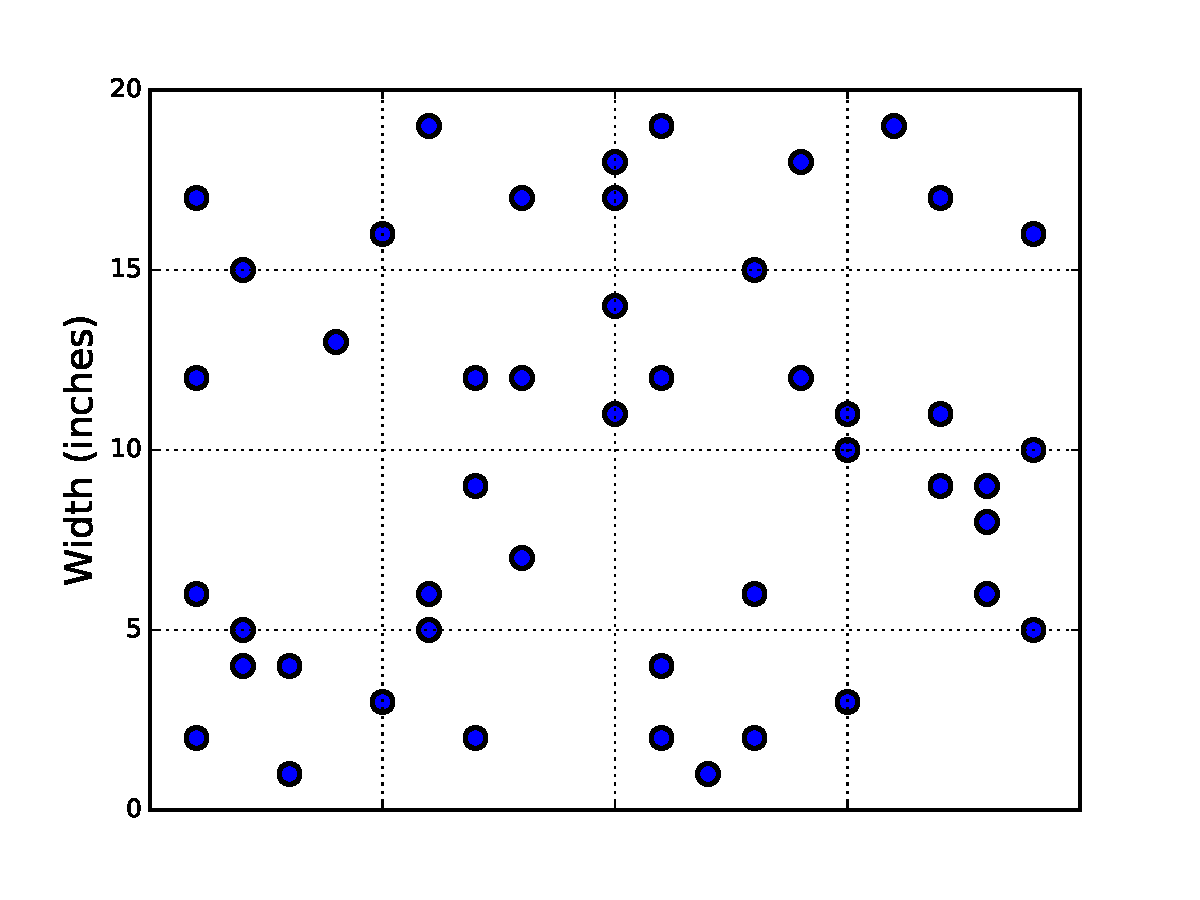
\includegraphics[width=\linewidth]{figures/scatter_1.pdf}
\end{subfigure}
%
\begin{subfigure}{.495\textwidth}
    \centering
    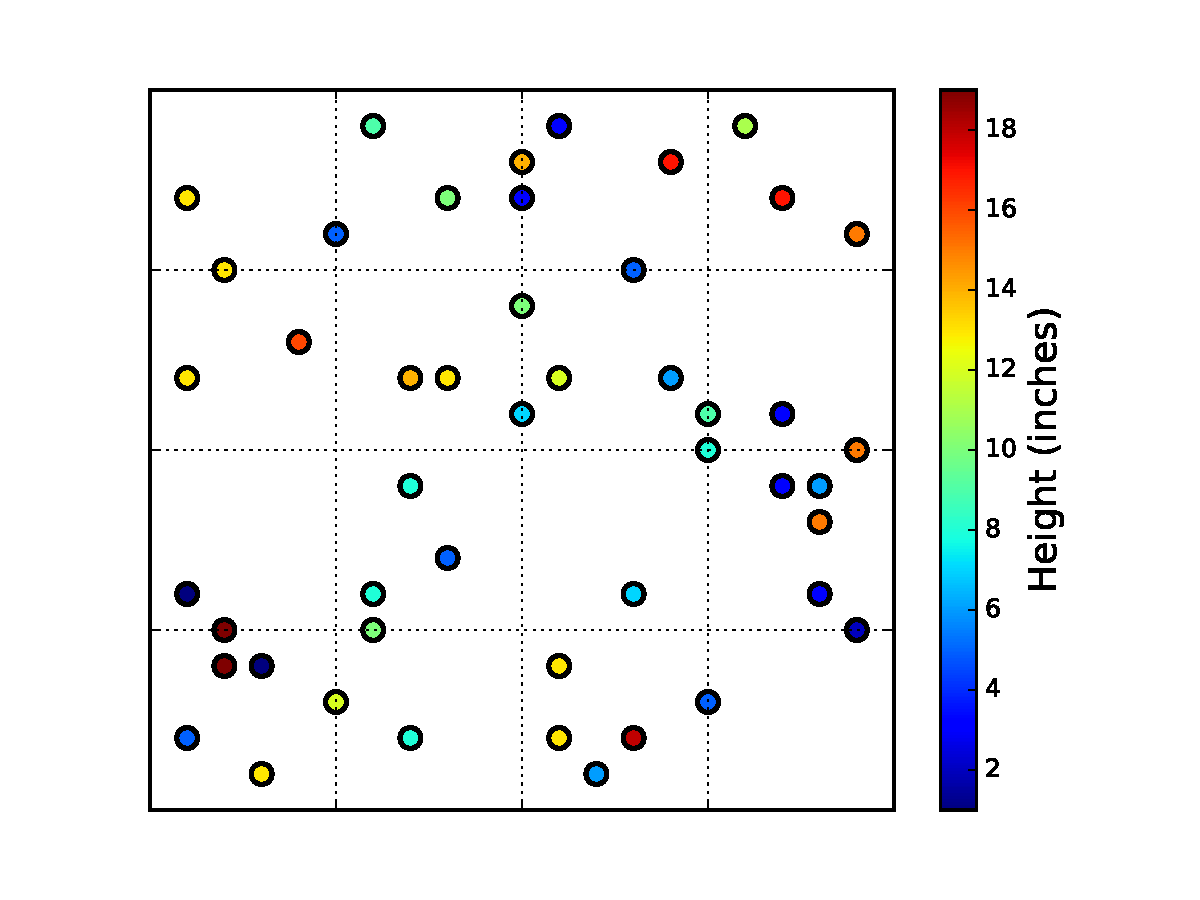
\includegraphics[width=\linewidth]{figures/scatter_2.pdf}
\end{subfigure}
\\
\begin{subfigure}{.495\textwidth}
    \centering
    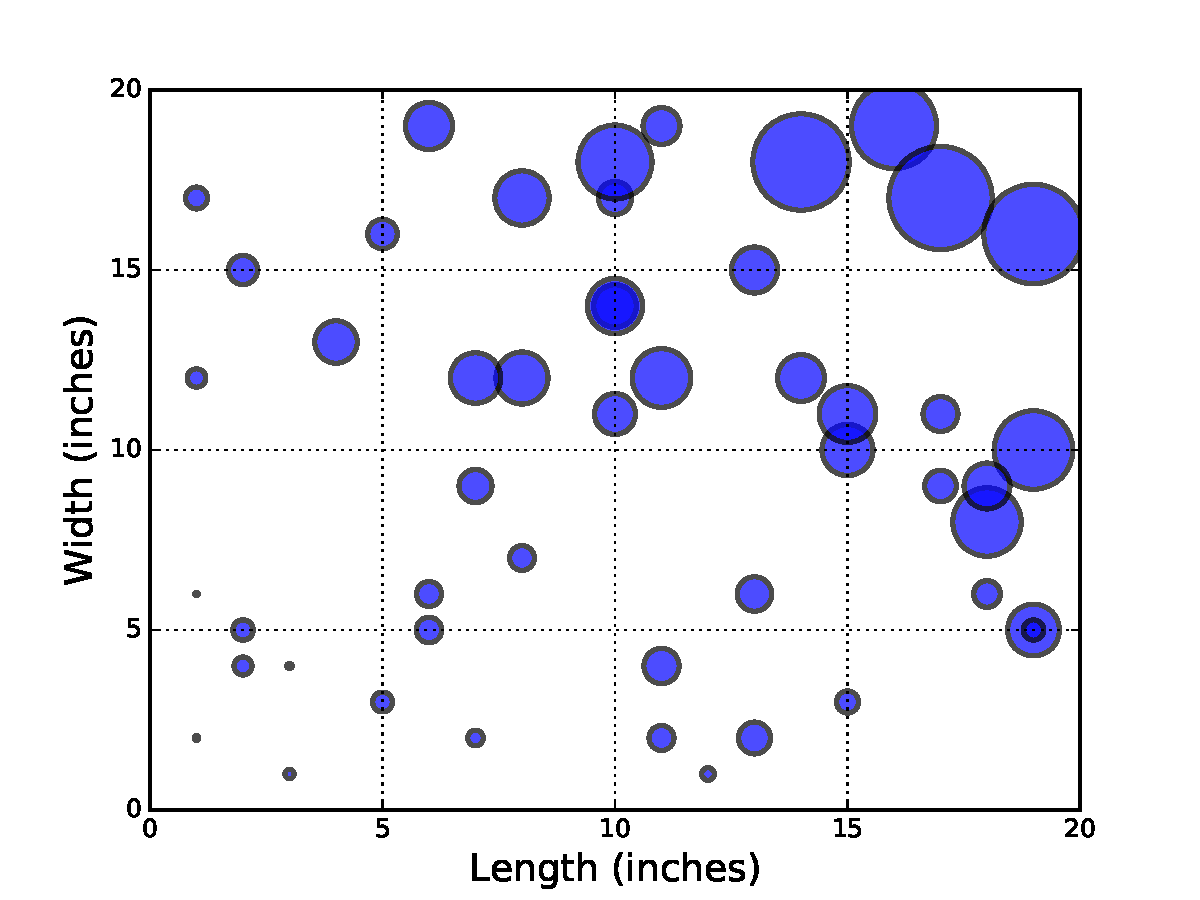
\includegraphics[width=\linewidth]{figures/scatter_3.pdf}
\end{subfigure}
%
\begin{subfigure}{.495\textwidth}
    \centering
    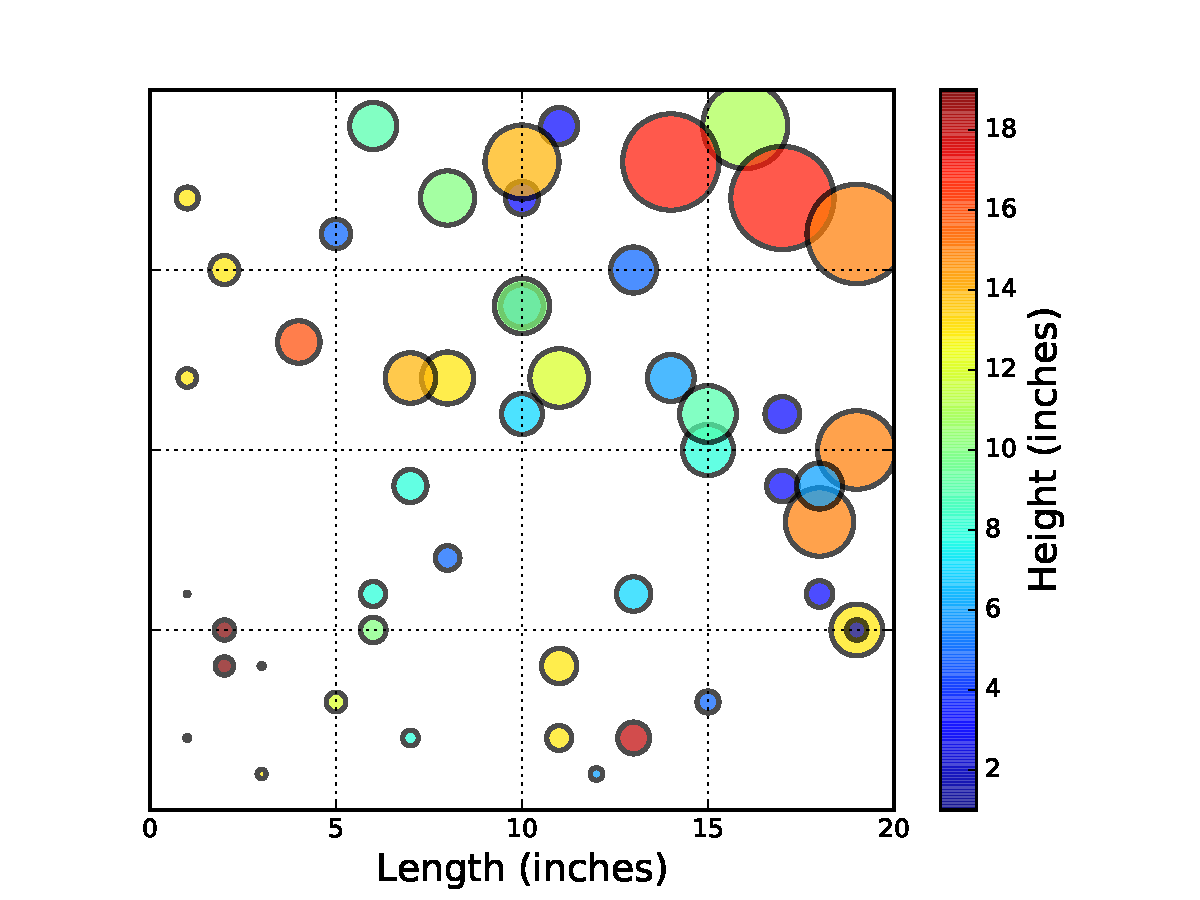
\includegraphics[width=\linewidth]{figures/scatter_4.pdf}
\end{subfigure}
\end{figure}

In scatter plots, connecting the points into a line plot usual results in extreme clutter.
A regression line, however, highlights a pattern in the data without overshadowing the actual data points.%
\footnote{See the Least Squares lab (QR 2), especially Problems 2–--4, for a refresher on regression lines.}

\begin{problem} % Scatter plots with visualizations.
The file \texttt{MLB.npy} contains measurements from over 1,000 recent Major League Baseball players, compiled by UCLA.\footnote{See \url{http://wiki.stat.ucla.edu/socr/index.php/SOCR_Data_MLB_HeightsWeights}.}
Each row in the array represents a different player; the columns are the player's height (in inches), weight (in pounds), and age (in years), in that order.

Describe the data with at least one scatter plot.
Your graph(s) should demonstrate whether height, weight, or age correlated with each other in the MLB.
Consider plotting linear regression lines to indicate trends.
\end{problem}

\subsection*{Histograms} % ----------------------------------------------------

A histogram partitions an interval into a number of bins and counts the number of values that fall into each bin.
Histograms are ideal for visualizing how unordered data in a single array is distributed over an interval.
If the data are draws from a probability distribution, a histogram approximates the distribution's probability density function (PDF).

\newpage

The following are important factors to consider when constructing a histogram.
%
\begin{itemize}
    \item What does the $x$-axis represent? How should it be labeled?
    \item Is a linear or a logarithmic scale more appropriate for the frequency axis?
    \item How many bins should be used? Over what range should the bins be?
    This is perhaps the most important question, as a histogram with too few or too many bins usually fails to give a clear view of the distribution.
\end{itemize}

% Use \li{plt.hist()} to create a histogram.
% The arguments \li{bins} and \li{<<range>>} specify the number of bins to draw and over what domain.

For most histograms, the most desirable insight is the general shape of the distribution.
The lines separating the bins, axis tick marks, and even the labels on the $y$ axis are all unnecessary (and potentially distracting) details.
Removing the lines between bins is easy: set the line width to $0$.
To ensure the gaps where the lines used to be are filled, specify the \li{histtype} as \li{"stepfilled"} (using \li{histtype="step"} will draw the outline without filling it in).
Finally, to get rid of extra markings on the axes, use \li{plt.tick_params()}.

A histogram can be converted into a line plot by using \li{np.histogram()}.
This function returns the number of values in each bin and the locations of the edges of the bins (in fact, \li{plt.hist()} employs this function).
Use the edges of the bins to calculate the center of the bins, then plot the bin centers against the frequency.

\begin{lstlisting}
# Get 10,000 random samples from a Beta distribution.
>>> data = np.random.beta(a=5, b=2, size=N)

>>> plt.subplot(131)                # Draw a regular histogram.
>>> plt.hist(data, bins=30)

>>> plt.subplot(132)                # Draw a clean histogram.
>>> plt.hist(data, bins=30, lw=0, histtype="stepfilled")
>>> plt.tick_params(left="off", top="off", right="off", labelleft="off")

>>> plt.subplot(133)                # Convert the histogram to a line plot.
>>> freq, bin_edges = np.histogram(data, bins=30)
>>> bin_centers = (bin_edges[:-1] + bin_edges[1:])/2.
>>> plt.plot(bin_centers, freq, 'k-', lw=4)
>>> plt.tick_params(left="off", top="off", right="off", labelleft="off")
\end{lstlisting}

\begin{figure}[H] % Cleaning up a histogram.
\centering
\begin{subfigure}{.325\textwidth}
    \centering
    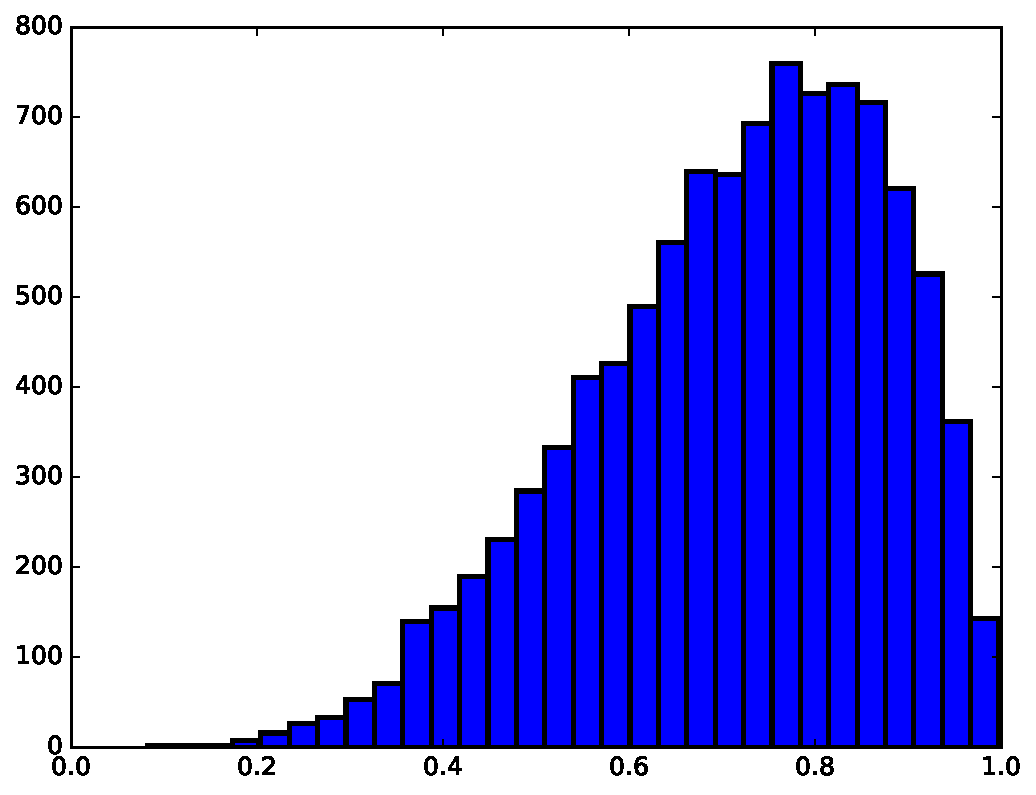
\includegraphics[width=\linewidth]{figures/histogram_2.pdf}
\end{subfigure}
%
\begin{subfigure}{.325\textwidth}
    \centering
    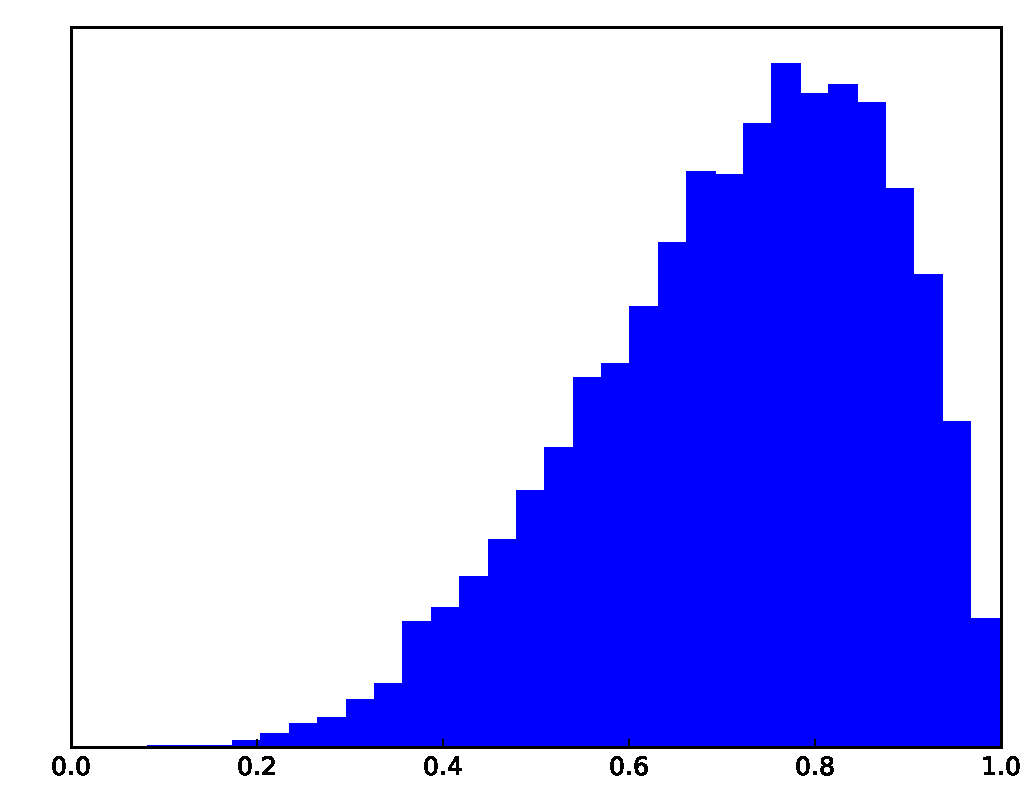
\includegraphics[width=\linewidth]{figures/histogram_3.pdf}
\end{subfigure}
%
\begin{subfigure}{.325\textwidth}
    \centering
    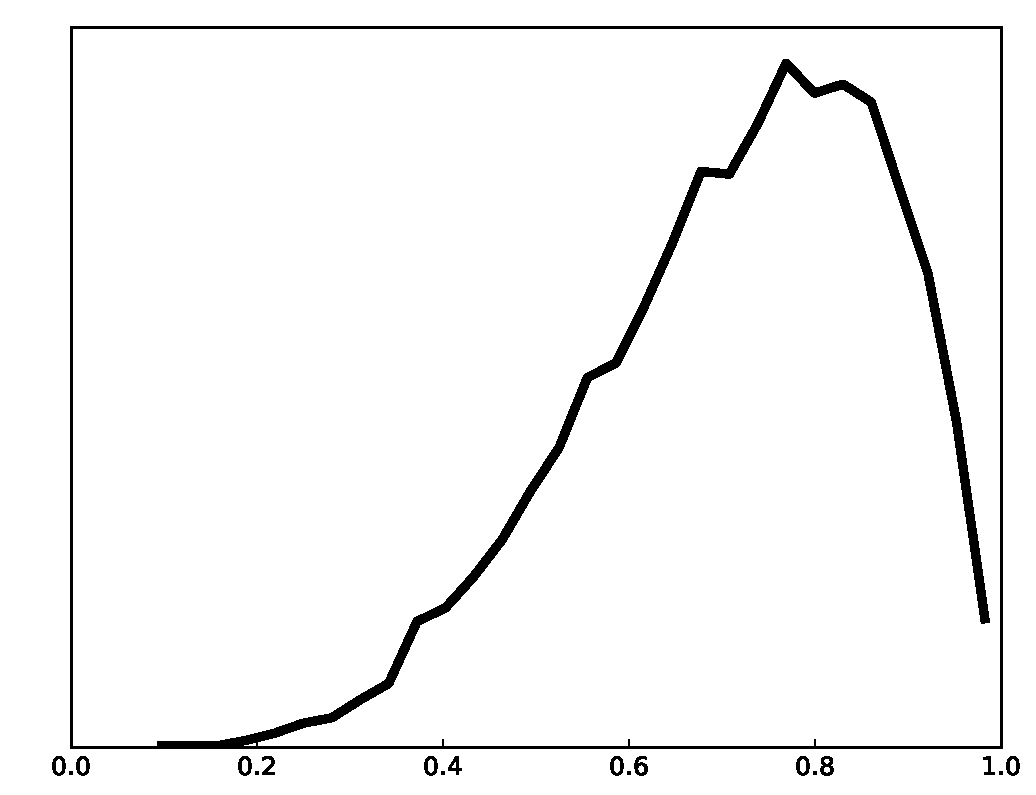
\includegraphics[width=\linewidth]{figures/histogram_4.pdf}
\end{subfigure}
\end{figure}

Finally, if the frequency domain is better visualized on a logarithmic scale, use \li{log=True} as an argument to \li{plt.hist()}.
This is the histogram equivalent of using \li{plt.semilogy()} for line or scatter plots.

\begin{warn} % Line plots versus histograms.
Line plots should \textbf{not} be used for data that has no natural progression.
For example, consider a collection of random draws from a statistical distribution.
In this case, a plain line plot is completely useless, because consecutive random draws are completely unrelated.
A histogram, on the other hand, provides an approximation of the distribution's probability density function.

\begin{lstlisting}
# Get 1,000 random samples from the standard normal distribution.
>>> data = np.random.normal(size=1000)

>>> plt.subplot(121)                # Regular line plot of the data.
>>> plt.plot(data)

>>> plt.subplot(122)                # Histogram of the data.
>>> plt.hist(data, bins=30)
\end{lstlisting}

\begin{figure}[H] % line plot versus a histogram.
\centering
\begin{subfigure}{.496\textwidth}
    \centering
    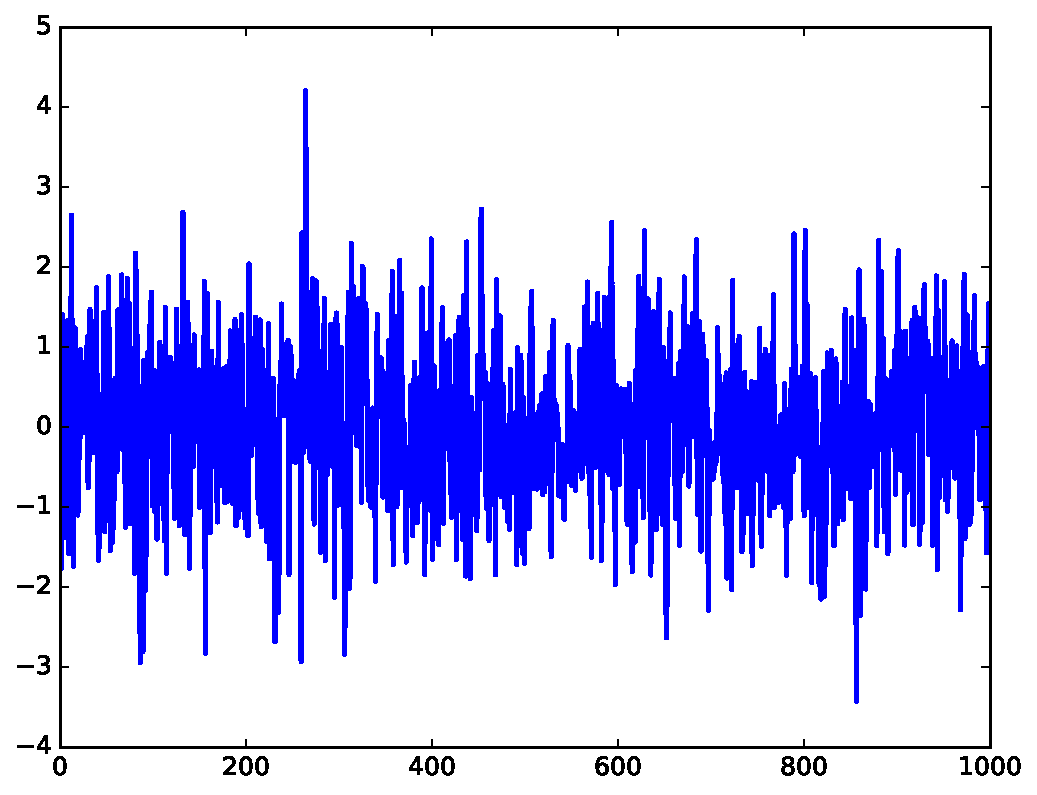
\includegraphics[width=\linewidth]{figures/histogram_1_bad.pdf}
\end{subfigure}
%
\begin{subfigure}{.49\textwidth}
    \centering
    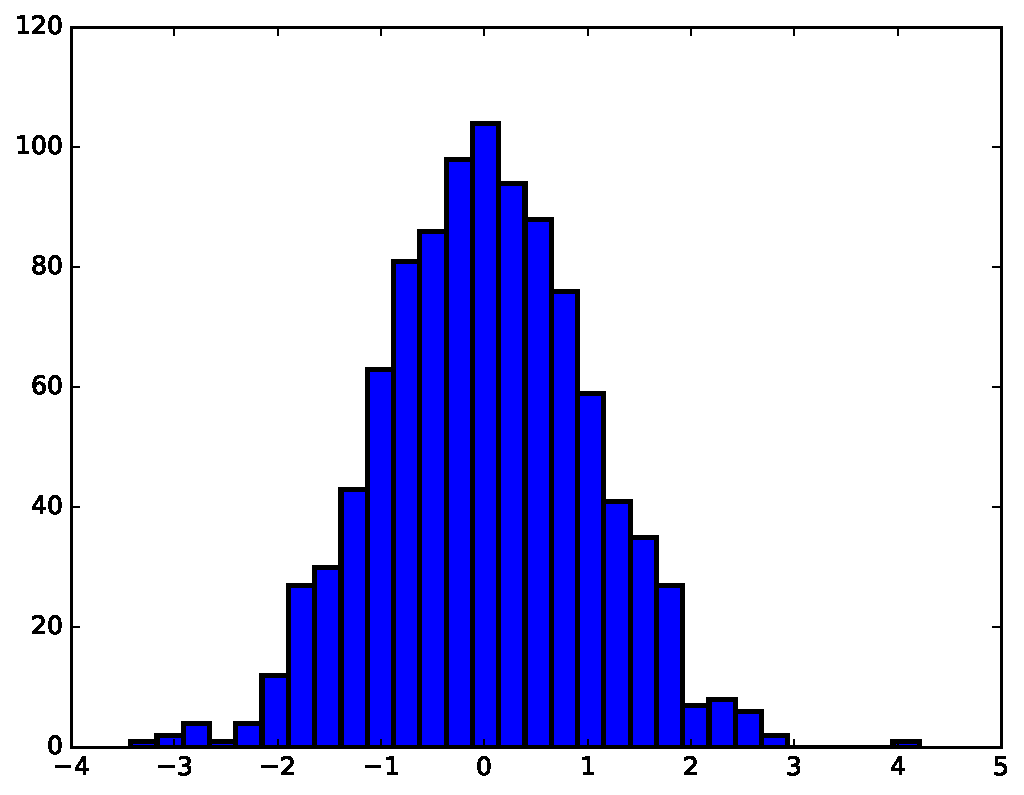
\includegraphics[width=\linewidth]{figures/histogram_1_good.pdf}
\end{subfigure}
\end{figure}
\end{warn}

\begin{problem} % Earthquake data
The file \texttt{earthquakes.npy} contains data from over 17,000 earthquakes between 2000 and 2010 that were at least a 5 on the Richter scale.\footnote{See \url{http://earthquake.usgs.gov/earthquakes/search/}.}
Each row in the array represents a different earthquake;
the columns are the earthquake's date (as a fraction of the year), magnitude (on the Richter scale), longitude, and latitude, in that order.

Because each earthquake is a distinct event, a good way to start visualizing this data might be a scatter plot of the years versus the magnitudes of each earthquake.

\begin{lstlisting}
>>> year, magnitude, longitude, latitude = np.load("earthquakes.npy").T
>>> plt.plot(year, magnitude, '.')
>>> plt.xlabel("Year")
>>> plt.ylabel("Magnitude")
\end{lstlisting}

\begin{figure}[H] % Bad visualization: earthquake data, year vs magnitude.
    \centering
    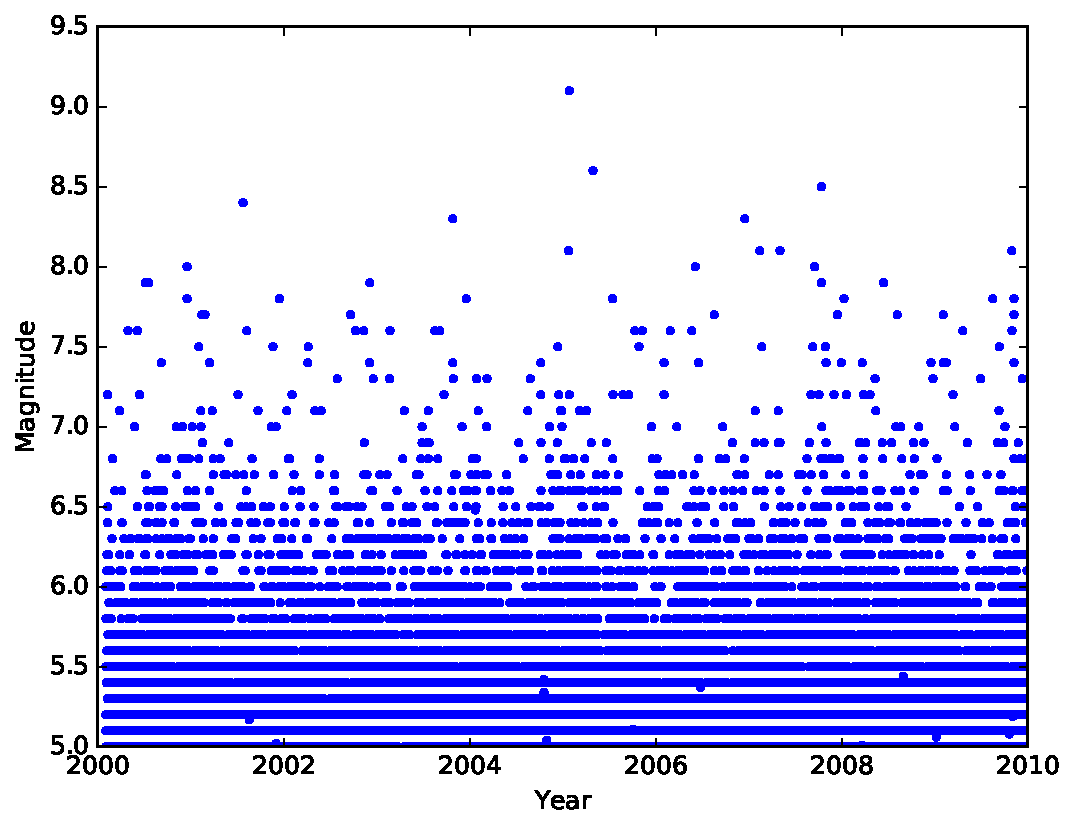
\includegraphics[width=.7\textwidth]{figures/earthquake.pdf}
\end{figure}

Unfortunately, this plot communicates very little information because the data is so cluttered.
Describe the data with two or three better visualizations, including line plots, scatter plots, and histograms as appropriate.
Your plots should clearly answer the following questions:
\begin{enumerate}
    \item How many earthquakes happened every year?
    \item How often do stronger earthquakes happen compared to weaker ones?
    \item Where do earthquakes happen? Where do the strongest earthquakes happen?
    \\(Hint: Use \li{plt.axis("equal")} to fix the aspect ratio, which may improve comparisons between longitude and latitude.)
\end{enumerate}
\end{problem}

\subsection*{Heat Maps and Contour Plots} % -----------------------------------

Let $f:\mathbb{R}^2\rightarrow\mathbb{R}$ be a scalar-valued function on a 2-dimensional domain.
A heat map of $f$ assigns a color to each $(x,y)$ point in the domain based on the value of $f(x,y)$, while a contour plot is a drawing of the level curves of $f$.
A filled contour plot, which colors in the sections between the level curves, is a discretized version of a heat map.

Consider the following questions when plotting a heat map or contour plot:
%
\begin{itemize}
    \item Is the domain sufficiently refined?
    \item Which color scheme is most clear and effective?
    \item How many / which contour lines should be drawn, if any?
    \item Is a linear or a logarithmic scale more appropriate for the color?
\end{itemize}

It is often sufficient to choose a fixed number of level curves, then let Matplotlib space the curves out evenly.
However, it is sometimes better to strategically specify the curves.
Consider, for example, the function $f(x,y) = y^2 - x^3 + x^2$ on the domain $[-\frac{3}{2}, \frac{3}{2}] \times [-\frac{3}{2}, \frac{3}{2}]$.
This function has a large basin around the origin.
Since $f(0,0) = 0$, plotting several level curves close to $0$ reveals the topography of the basin.

\begin{lstlisting}
# Construct a 2-D domain with np.meshgrid() and calculate f on the domain.
>>> x = np.linspace(-1.5, 1.5, 200)
>>> X, Y = np.meshgrid(x, x.copy())
>>> Z = Y**2 - X**3 + X**2

>>> plt.subplot(221)                # Plot a heat map of f.
>>> plt.pcolormesh(X, Y, Z, cmap="viridis")
>>> plt.colorbar()

>>> plt.subplot(222)                # Plot a contour map with 6 level curves.
>>> plt.contour(X, Y, Z, 6, cmap="viridis")
>>> plt.colorbar()

>>> plt.subplot(223)                # Plot a filled contour map with 12 levels.
>>> plt.contourf(X, Y, Z, 12, cmap="viridis")
>>> plt.colorbar()

>>> plt.subplot(224)                # Plot specific level curves and a heat map.
>>> plt.contour(X, Y, Z, [-1, -.25, 0, .25, 1, 4], colors="white")
>>> plt.pcolormesh(X, Y, Z, cmap="viridis")
>>> plt.colorbar()
\end{lstlisting}

\begin{figure}[H] % Heat maps and contour plots.
\centering
\begin{subfigure}{.495\textwidth}
    \centering
    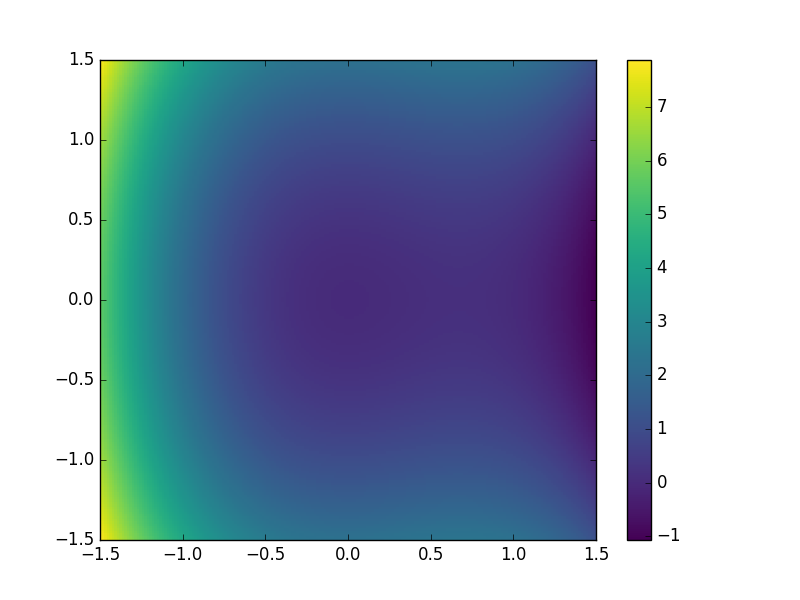
\includegraphics[width=\linewidth]{figures/heatmap_1.png}
\end{subfigure}
%
\begin{subfigure}{.495\textwidth}
    \centering
    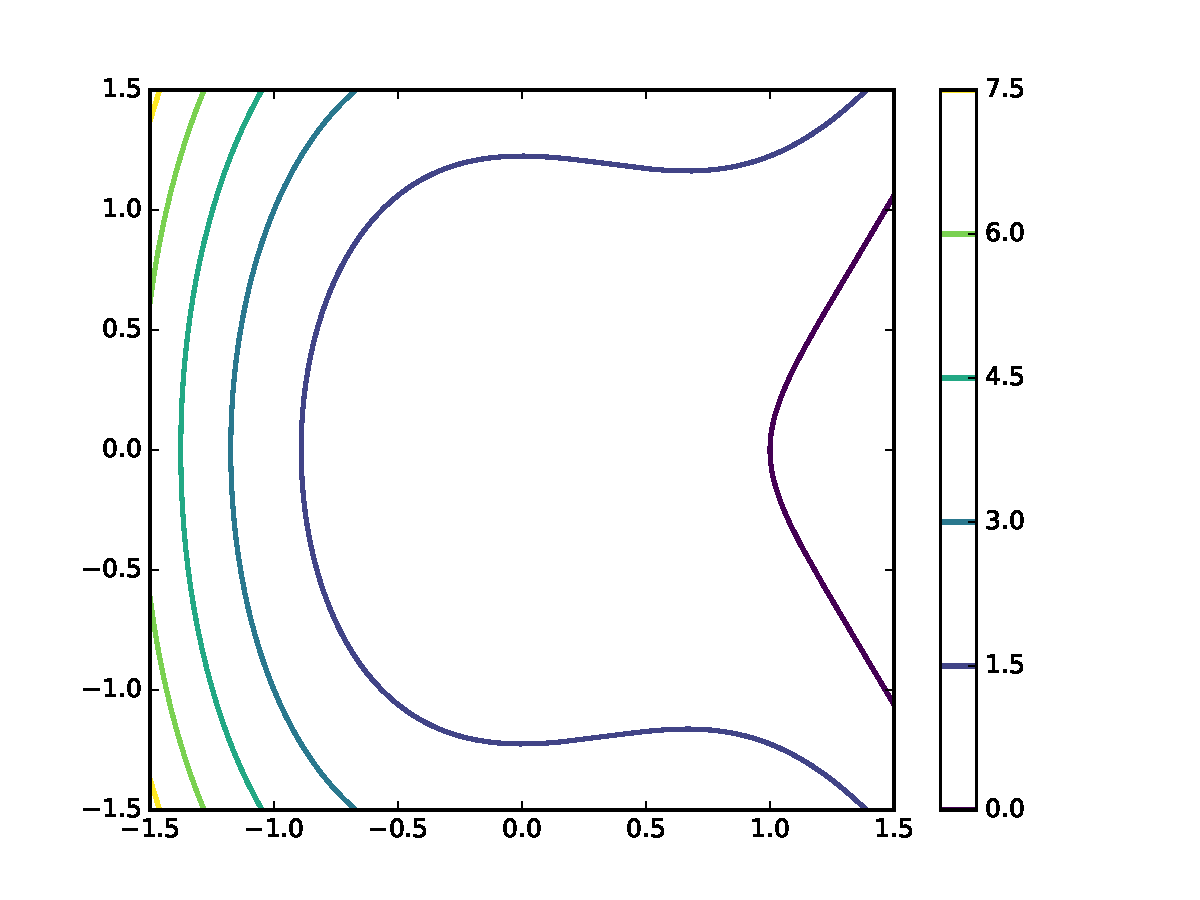
\includegraphics[width=\linewidth]{figures/contour_1.pdf}
\end{subfigure}
\\
\begin{subfigure}{.495\textwidth}
    \centering
    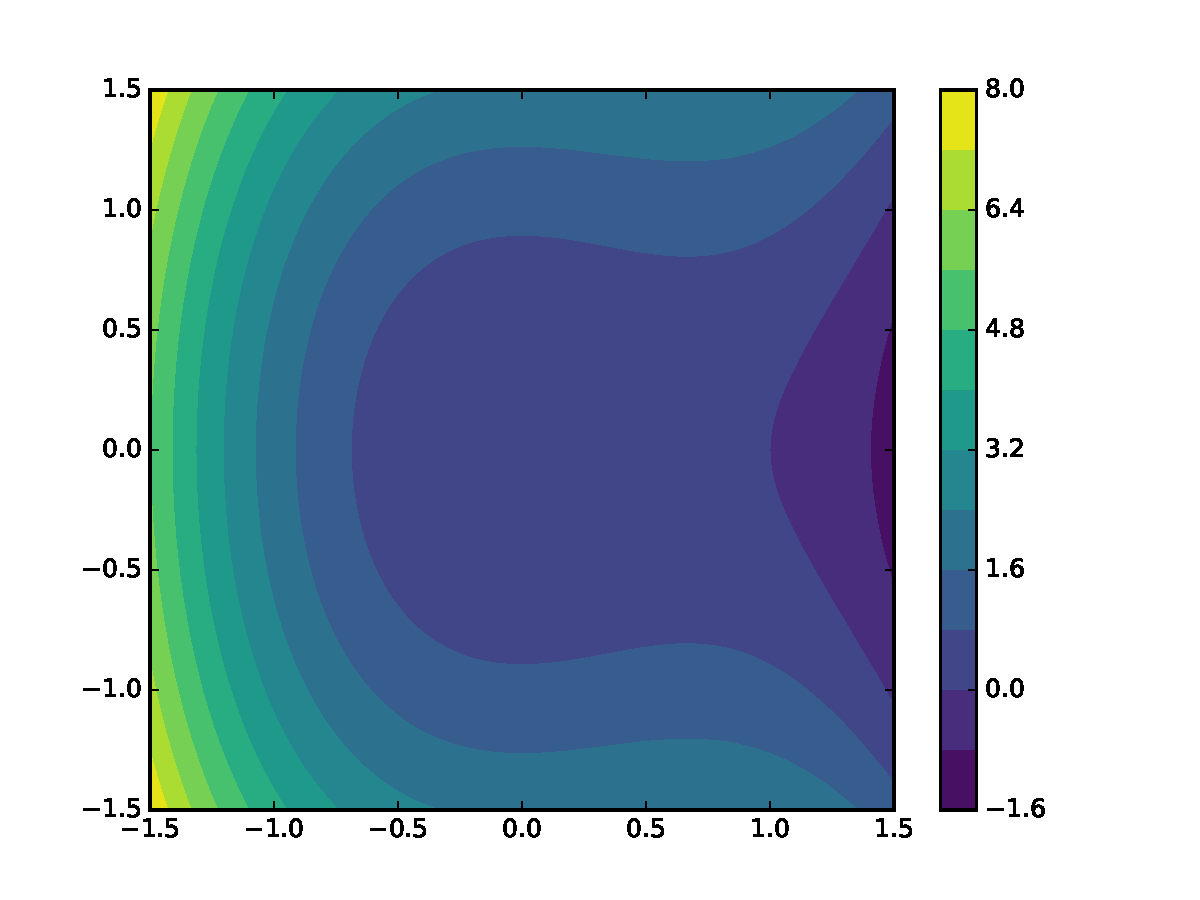
\includegraphics[width=\linewidth]{figures/contour_2.pdf}
\end{subfigure}
%
\begin{subfigure}{.495\textwidth}
    \centering
    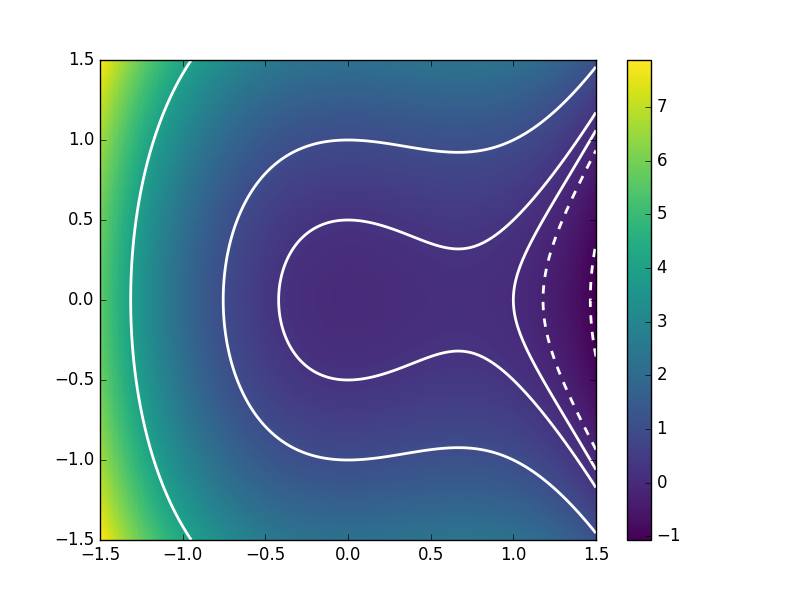
\includegraphics[width=\linewidth]{figures/heatmap_2.png}
\end{subfigure}
\end{figure}

There are two main kinds of color maps: sequential and diverging.
Sequential color maps, like \li{"hot"} and \li{"cool"}, transition very gradually between two colors; diverging color maps, like \li{"seismic"} and \li{"coolwarm"}, transition very rapidly from one color to another at the mean value.
When in doubt, use \li{"viridis"} or \li{"plasma"}, two specialized sequential color schemes.
For the complete list of Matplotlib color maps, see \url{http://matplotlib.org/examples/color/colormaps_reference.html}.

The color map can also be changed to a log scale by using the keyword argument \li{norm=matplotlib.colors.LogNorm()} (this works for \li{plt.scatter()} as well).
As an example, consider the same $f$ defined above on the larger domain $[-6,6]\times [-6,6]$.
Log scaling can only be done on arrays of all positive values, so we visualize $|f|$.

\begin{lstlisting}
>>> from matplotlib.colors import LogNorm

>>> x = np.linspace(-6, 6, 200)
>>> X, Y = np.meshgrid(x, x.copy())
>>> Z = np.<<abs>>(Y**2 - X**3 + X**2)

>>> plt.subplot(121)              # Plot a regular heat map of |f|.
>>> plt.pcolormesh(X, Y, Z, cmap="viridis")
>>> plt.colorbar()

>>> plt.subplot(122)              # Plot a filled contour plot with log scaling.
>>> plt.contourf(X, Y, Z, 6, cmap="viridis", norm=LogNorm())
>>> plt.colorbar()
\end{lstlisting}

\begin{figure}[H] % Heat maps and contour plots.
\centering
\begin{subfigure}{.495\textwidth}
    \centering
    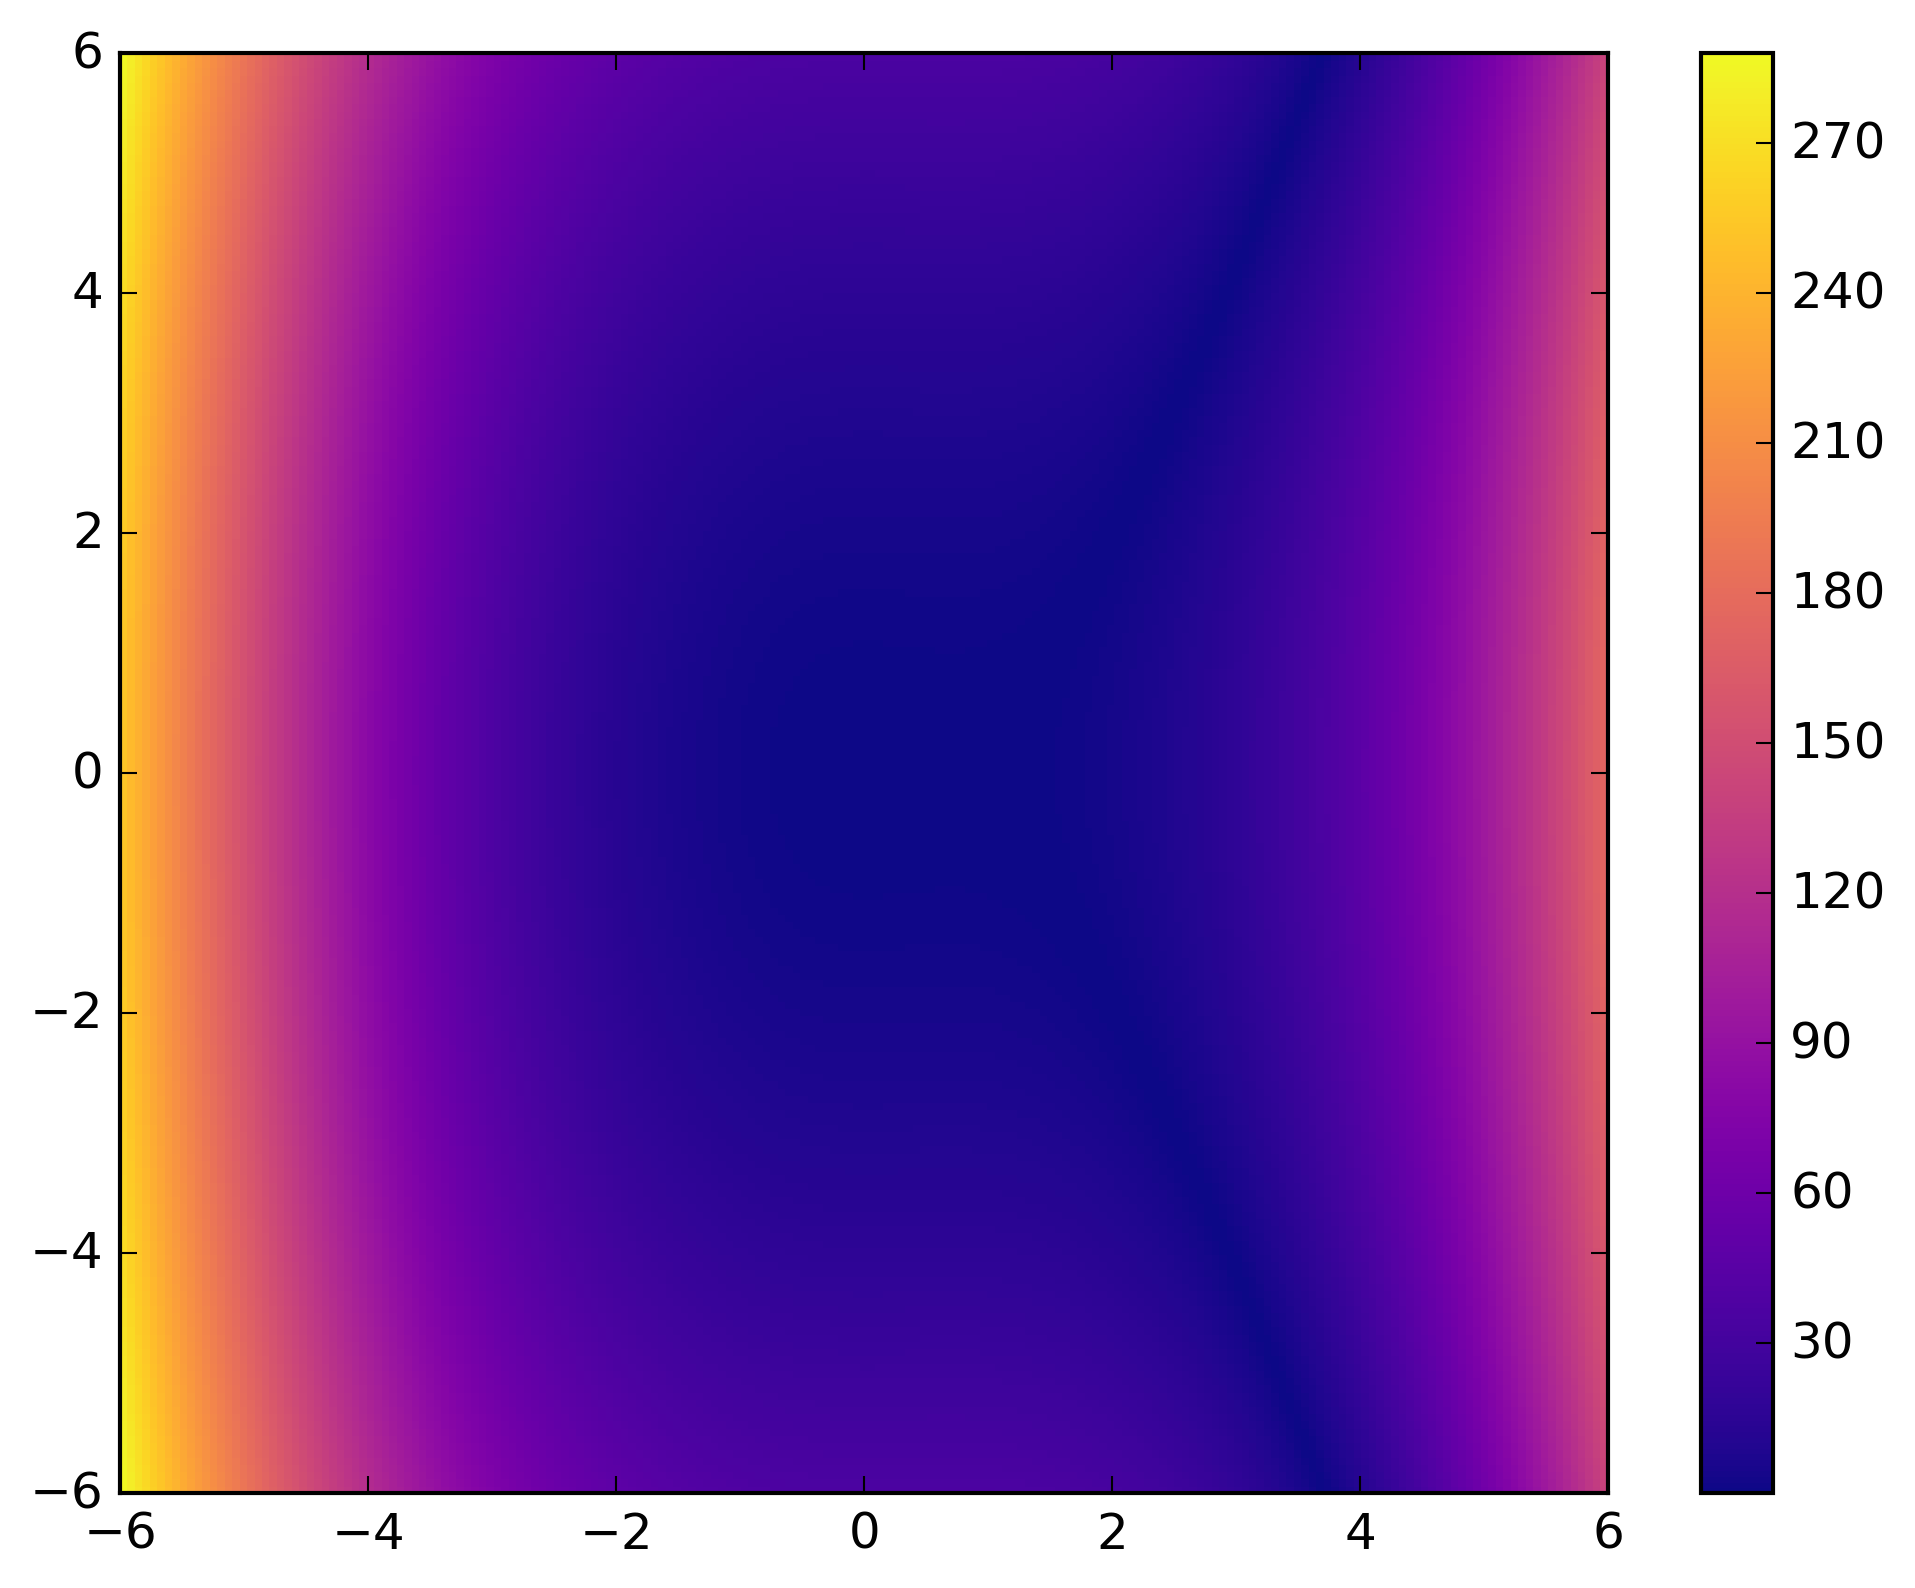
\includegraphics[width=\linewidth]{figures/heatmap_3.png}
\end{subfigure}
%
\begin{subfigure}{.495\textwidth}
    \centering
    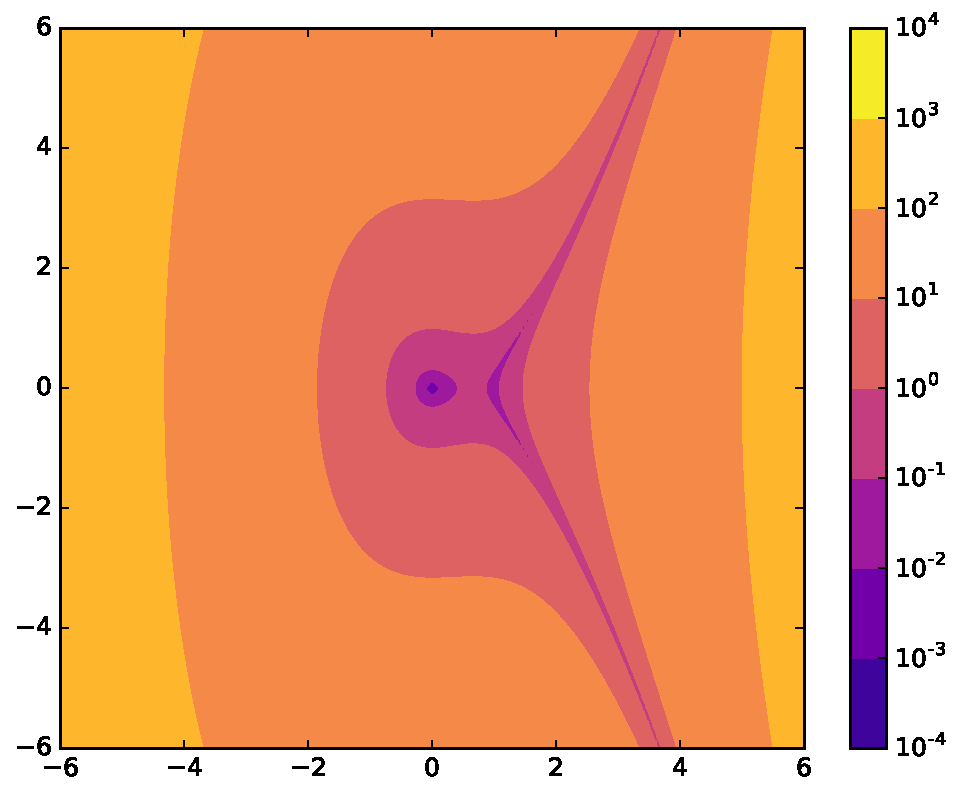
\includegraphics[width=\linewidth]{figures/contour_3.pdf}
\end{subfigure}
\end{figure}

\begin{problem} % Contour map problem. TODO: ROSENBROCK!!!
The \emph{Rosenbrock function} is defined as follows.
\[f(x,y) = (1-x)^2 + 100(y-x^2)^2\]
The minimum value of $f$ is $0$, which occurs at the point $(1,1)$ at the bottom of a steep, banana-shaped valley of the function.

Use heat maps and contour plots to visualize the Rosenbrock function in such a way that the minimum value, and the valley that it lies in, is apparent.
Consider plotting the minimizer $(1,1)$ on top of the plot as well.
\end{problem}

\subsection*{Bar Charts} % ----------------------------------------------------

A bar chart plots categorical data in a sequence of bars across an axis.
They are best for small sets of discrete, one-dimensional, categorical data.
Usually, a horizontal bar chart is preferred over a vertical bar chart because it's harder to read vertical labels than horizontal labels.

The data in a bar chart should be sorted in a logical way.
If the chart is being used to compare the values of different data points, it is best to sort by size; if the chart is being used to look up specific values, the labels should be sorted in a way that makes it easy to find specific values (for example, alphabetically).
Use \li{plt.bar()} or \li{plt.barh()} to create a bar chart in Matplotlib.

% TODO: improve this section.

Some kinds of visualizations, especially for categorical data, are popular even though they interfere with the reader's ability to interpret the displayed information.
For example, it is more difficult to see the differences in a pie chart than on a bar chart since differences in area are more difficult to detect than differences in length.
By the same logic, a stacked bar chart is almost always inferior to a side-by-side bar chart.

It may also be tempting to stylize a visualization by adding extra icons or pictures or by making certain features look 3-D.
Anything in a plot that fails to communicate information or that misrepresents the data is called \emph{chartjunk}, a term coined by Edward Tufte.
Avoid making visualizations that are overly fancy or cluttered with chartjunk;
Visualizations are at their best when they are as simple as possible, allowing the reader to easily interpret the information.

% This code created the top right bar chart.
% Why reverse the labels?
\begin{lstlisting}
>>> labels = ["Spam", "Eggs", "Ham", "Sausage", "Bacon",
...                         "Baked beans","Lobster thermidor"]
>>> lengths = [10, 11, 18, 19, 20, 21, 22]
>>> positions = np.arange(7)+.5
>>> plt.barh(positions, lengths, align="center")
>>> plt.yticks(positions, labels[::-1])
\end{lstlisting}

\begin{figure}[H] % Pie chart --> Bar chart
\centering
\begin{subfigure}{.495\textwidth}
    \centering
    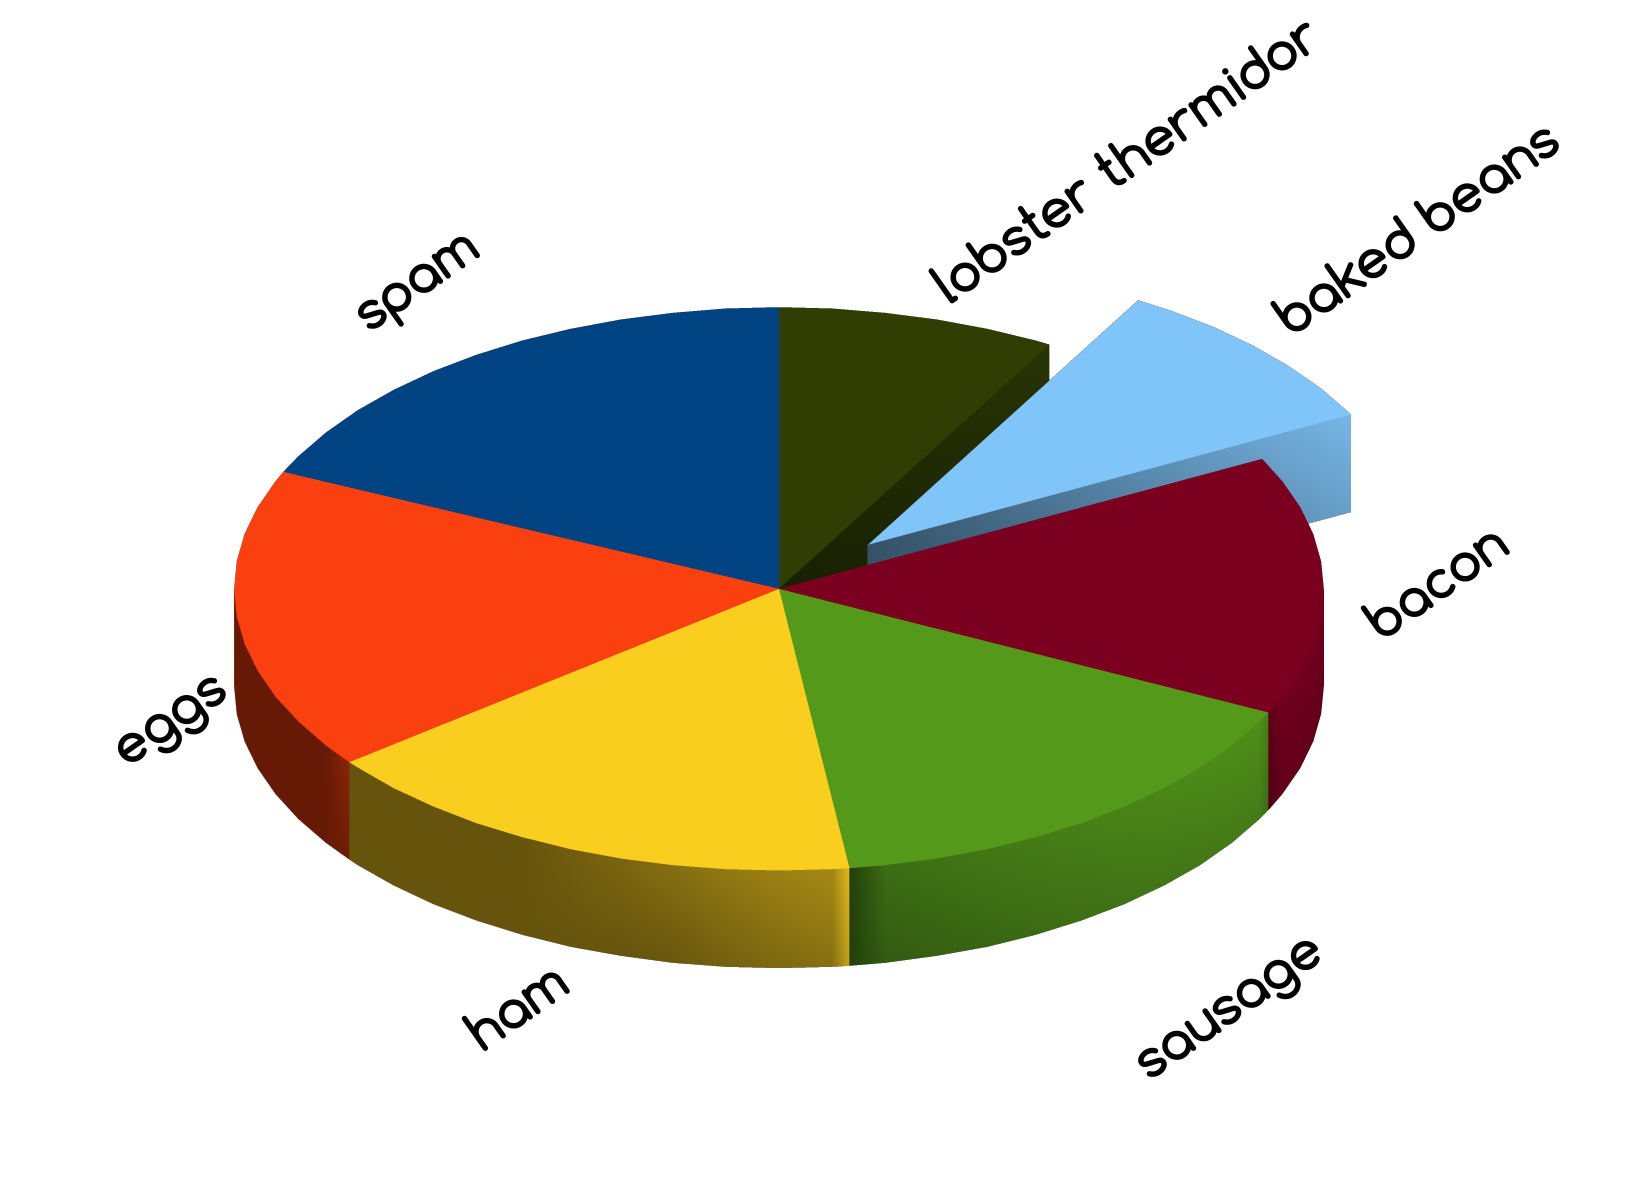
\includegraphics[width=\textwidth]{bad_pie_chart.png}
\end{subfigure}
%
\begin{subfigure}{.495\textwidth}
    \centering
    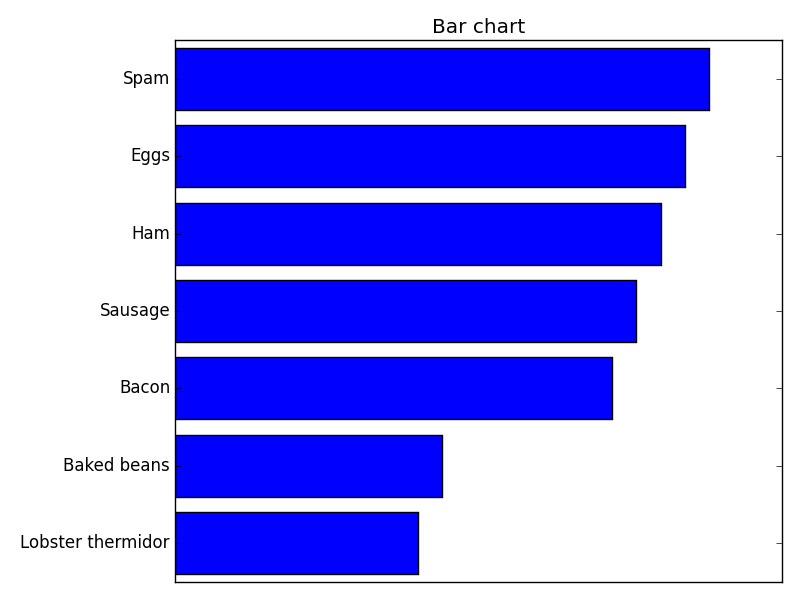
\includegraphics[width=\textwidth]{bar_chart_horizontal_sorted.png}
\end{subfigure}
\caption{Transforming the horrendous 3-D pie chart on the left into the horizontal bar chart on the right both simplifies and clarifies the information.}
\label{fig:pievsbar}
\end{figure}

\begin{problem}
The file \texttt{countries.npy} contains some information about 20 countries.
Each row in the array is a country; the columns are the population (in millions of people), the 2015 GDP (in billions of US dollars), the average male height (in centimeters), and the average female height (in centimeters), in that order.%
\footnote{
See \url{https://en.wikipedia.org/wiki/List_of_countries_by_GDP_(nominal)}, \url{http://www.averageheight.co/}, and
\url{https://en.wikipedia.org/wiki/List_of_countries_and_dependencies_by_population}.
}

Visualize the data in at least four plots, using at least one scatter plot, one histogram, and one bar chart.
\end{problem}

\begin{comment} % Find a place for this.
\begin{figure}[h] % Choose an ethical scale and window.
\centering
\begin{subfigure}{.45\textwidth}
\centering
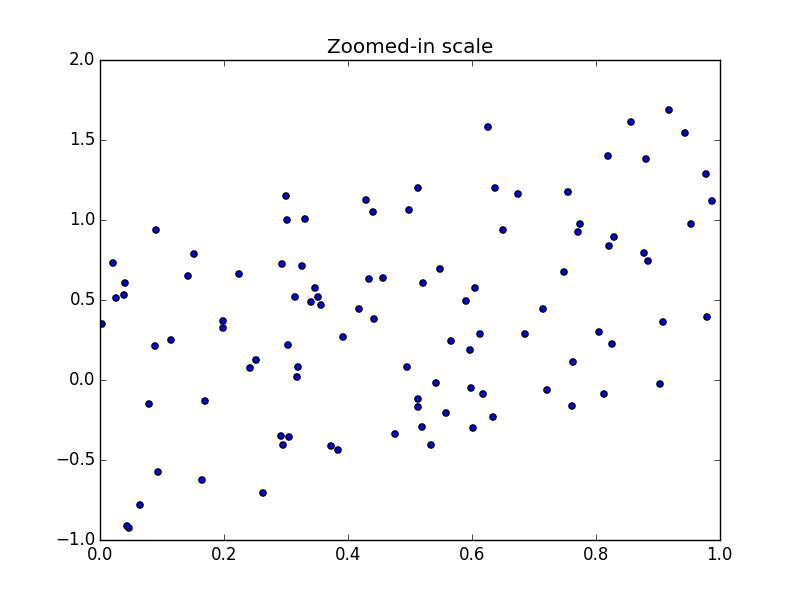
\includegraphics[width=\textwidth]{scale_scatter_zoomed_in.png}
\end{subfigure}
\begin{subfigure}{.45\textwidth}
\centering
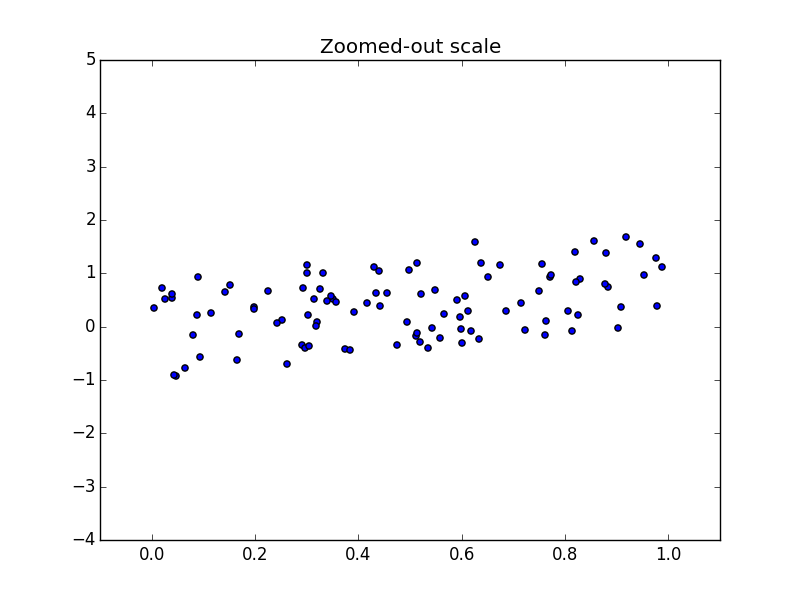
\includegraphics[width=\textwidth]{scale_scatter_zoomed_out.png}
\end{subfigure}
\caption{Scatter Plots. The data in both plots are the same but there appears to be a weaker
correlation in the first plot compared to the second.}
\label{fig:scatter_correlation}
\end{figure}

Scatter plots may reveal insights other than correlation.
Consider Figure \ref{fig:scatterquake} which plots earthquake data from the United States Geological Survey (USGS).
The USGS data began including earthquakes with magnitude 6.5 or greater; this is clearly seen
in the scatter plot of the entire dataset.
Plots like this may also reveal errors in the dataset that are harder to detect in a table of values.
\end{comment}

\begin{comment} % This needs to go somewhere else. Conclusion?
Understanding a data set through visualizations is an iterative process.
Start with an initial visualization---usually a broad overview---and examine the data, then adjust the visualization or create other visualizations based on what you observe.
Ask the following questions as you search for insights:
%
\begin{enumerate}
\item Does the data make sense?
\item Would a different visualization communicate more information?
\item Would visualizing a subset of the data provide more information?
\item Would transforming the data reveal a hidden pattern?
\end{enumerate}
\end{comment}

\begin{comment} % TODO: Add sections on box plots and hexbin plots.
\subsection*{Additional Material} % ===========================================

There are many software packages that facilitate the visual exploration of data.
One Python library is Glue (see \cite{glue}).

Some packages for making nicer looking plots include \li{Seaborn} and \li{prettyplotlib}.

For more about visualization of data, we highly recommend the following books and websites:

% TODO: get full refs for the following

\begin{itemize}
    \item \emph{How to Lie with Statistics} by Darrell Huff (1954)
    \item \emph{Envisioning Information} by Edward Tufte
    \item \emph{The Visual Display of Quantitative Information} by Edward Tufte (2nd edition)
    \item \emph{Beautiful Evidence} by Edward Tufte
    \item \emph{Now you see it} by Stephen Few
    \item \url{http://www.informationisbeautiful.net/}
\end{itemize}
\end{comment}
